\newpage
\section{Data analysis and interpretation}

\subsection{Participants}

The sample consisted of 61 fictional under-graduate students from a University in Perth, Western Australia who responded to a survey regarding their Facebook use. 

Out of the 61 observations, five were excluded from the dataset with NA responses. Three observations were excluded with responses to the questionnaire as ``0'' (zero). The dataset was then screened for outliers, excluding two observations with reported Facebook logins greater than 50 per week. One observation was excluded, with reported hours spent Facebook greater than 50 per week. Finally, two observations were excluded, with reported number of close friends greater than 70.

This resulted in a final sample of 48 Facebook users, 3 female, 45 male (M = 0.938, SD = 0.2446) between the ages of 17 to 29 (M = 20.6, SD = 3.206543). Gender is coded as 0 = female and 1 = male in the dataset.

\subsection{Survey}

Each participant filled out a survey which consisted of 10 questions. The first section included questions about the participants demography, requesting their age and sex. 

The second section included questions regarding the amount of Facebook use, requesting self-reported estimates on how many Facebook logins per week, and hours spent per week on Facebook. 

The third section included questions regarding the participant's social networking and connection, requesting self-reported estimates on how many Facebook friends they have, how many offline close friends they have, and a 5 point Likert-style scale opinion of their own sociability; 1 = strongly disagree, 5 = strongly agree. 

The fourth and final section included personality surveys, measuring extraversion, self-esteem and social anxiety. Extraversion was measured through a personality test of 25 items, the scores of which were converted to an integer value between 1 and 25. A lower value suggests introversion and a higher value suggests extraversion. Self esteem was measured using a Rosenberg self esteem scale survey of 10 items. The scale ranges between 0 to 30, with scores between 15 to 25 considered normal, and scores below 15 suggesting low self esteem. Social anxiety was measured using a Liebowitz Social Anxiety Scale survey of 24 items, with scores between 55 to 65 suggesting moderate social phobia, scores between 65 to 80 suggesting marked social phobia, 80 to 95 suggesting severe social phobia and scores greater than 95 suggesting very severe social phobia.

This research paper aims to explore the relationship between gender and network size, and the relationship between gender and amount of time spent on Facebook. As such, the following measured variables from the survey have been selected for this research:

\begin{itemize}
\item Gender
\item Facebook friends (FB friends)
\item Close friends
\item Sociability
\item Facebook hours
\end{itemize}

\subsection{Descriptive statistics}

Table 1 provides centrality measures of the selected variables.

\begin{table}[H]
\centering
\caption{Measures of centrality}
\begin{tabular}{l|l|l|l|l|l|l}
Variable      & Mean   & Median & Mode & Std. Dev & Skew    & Kurt      \\ \hline
Gender        & 0.9375 & 1      & 1    & 0.2446   & -3.502  & 10.49     \\ \hline
FB Friends    & 290.7  & 275    & 242  & 176.001  & 0.7959  & 0.04759   \\ \hline
Close Friends & 21.73  & 19     & 23   & 12.29    & 0.9668  & 0.1483    \\ \hline
Sociability   & 3.667  & 4      & 4    & 0.7532   & -0.5633 & -0.008646 \\ \hline
\end{tabular}
\end{table}

%As shown in the table above, and in the histograms and q-q plots to follow, all the variables are non-normally distributed. Therefore, non-parametric inferential tests will be used.

It is worth noting that men greatly outnumber women in this sample set by 15 to 1. Unfortunately, there is not enough female representation in the dataset to provide any meaningful conclusions in the tests to follow.

\subsubsection{Gender}

Figure 1 shows the histogram for gender. The blue curve overlay demonstates a non-normal distribution. Only non-parametric tests are applicable for this variable. As previously mentioned, men greatly outnumber women in this study, therefore, no meaningful conclusions can be made from the following tests.

\begin{figure}[H]
\centering
\caption{Histogram: Gender}
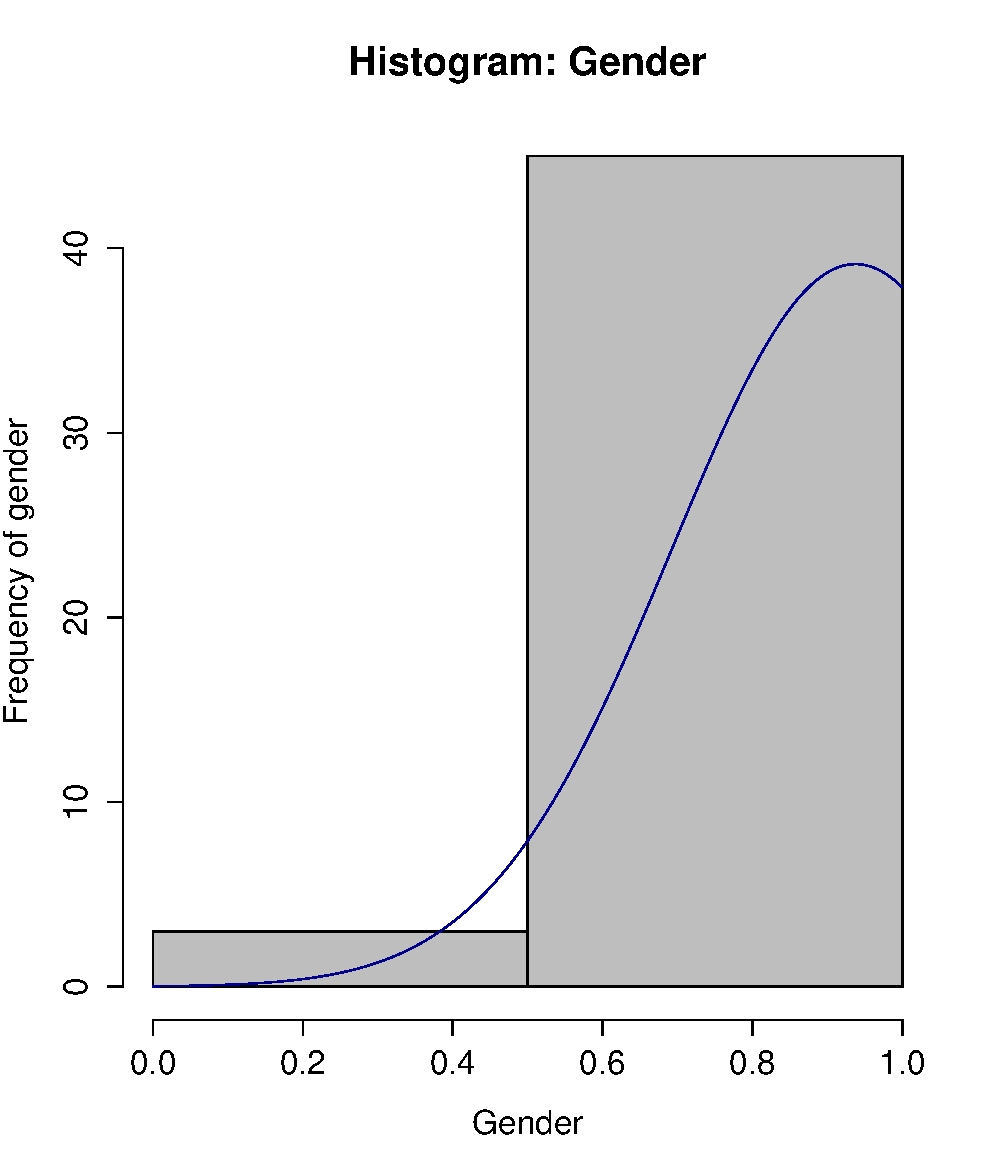
\includegraphics[scale=0.35]{./img/hist_gender.pdf}
\end{figure}

\newpage
\subsubsection{Facebook friends}

Figure 2 shows the histogram and normal q-q plot for Facebook friends. The blue curve overlay on the histogram demonstrates a non-normal distribution. The normal q-q plot also demonstrates a non-normal distribution, as the majority of data-points do not fall on the expected normal distribution line. Only non-parametric tests are applicable for this variable.

\begin{figure}[H]
\caption{Histogram and Normal Q-Q Plot: Facebook friends}
\centering
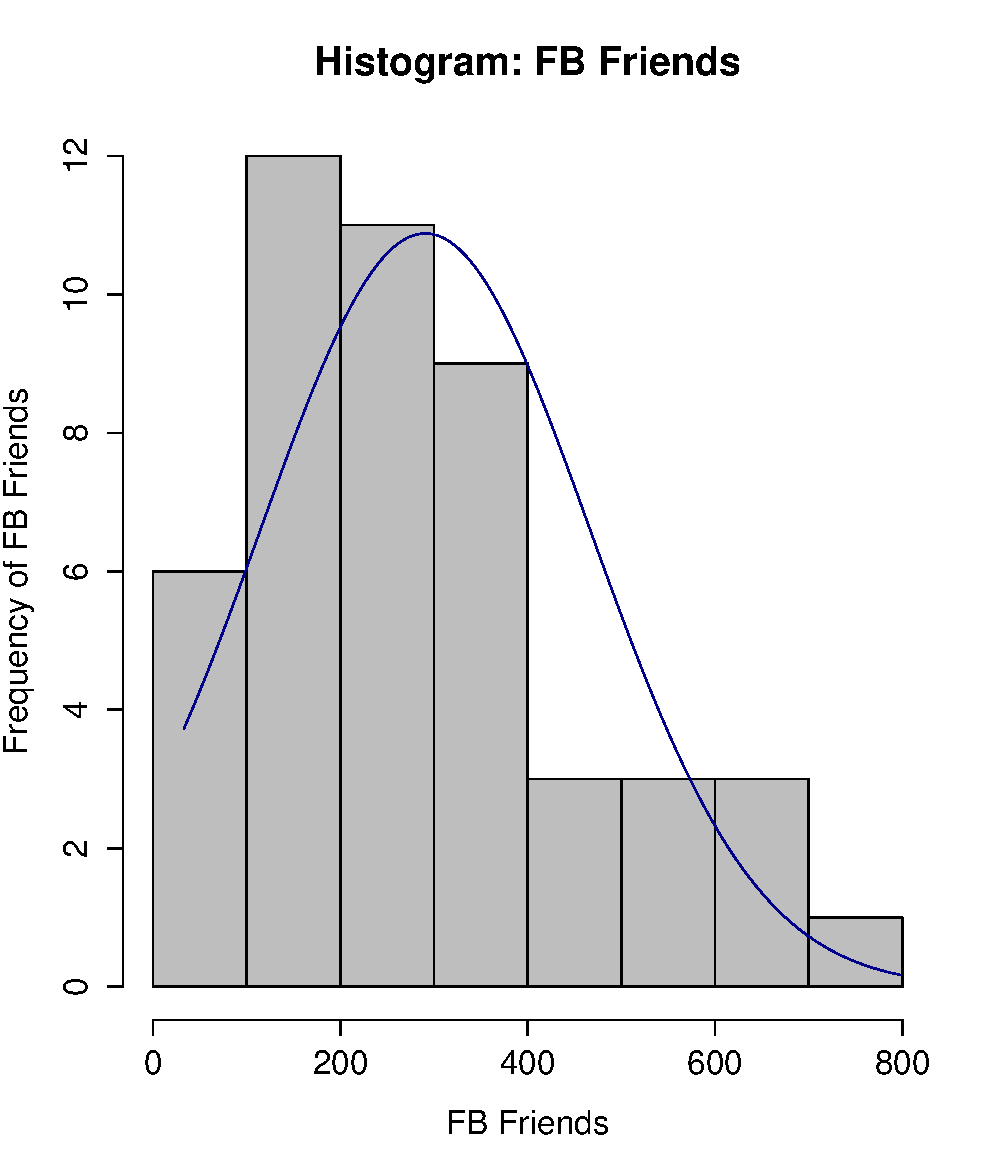
\includegraphics[scale=0.35]{./img/hist_fbfriends.pdf}
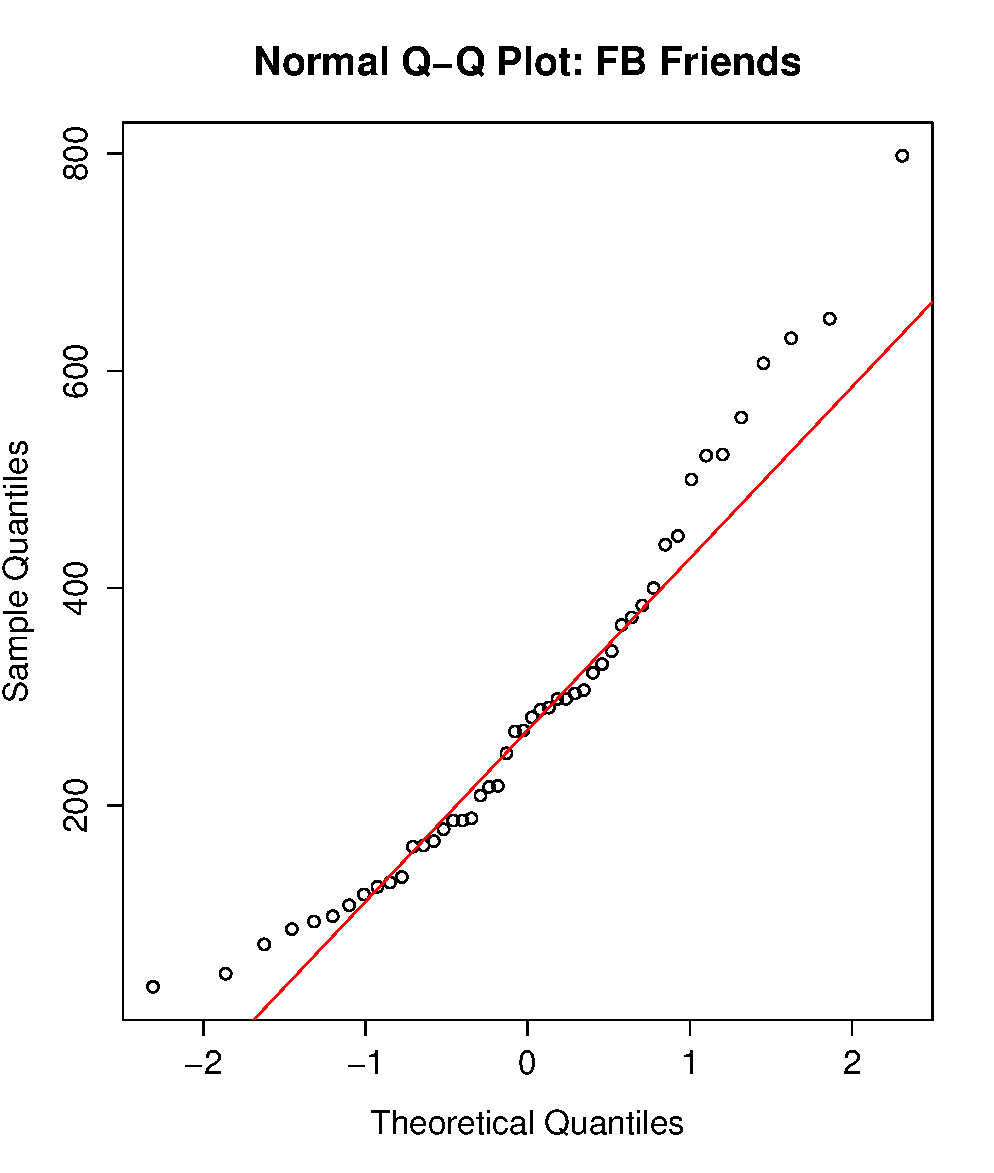
\includegraphics[scale=0.35]{./img/qqplot_fbfriends.pdf}
\end{figure}

\subsubsection{Close friends}

Figure 3 shows the histogram and normal q-q plot for close friends. The blue curve overlay on the histogram demonstrates a non-normal distribution. The normal q-q plot also demonstrates a non-normal distrbution, as the majority of data-points do not fall on the expected normal distribution line. Only non-parametric tests are applicable for this variable.

\begin{figure}[H]
\caption{Histogram and Normal Q-Q Plot: Facebook friends}
\centering
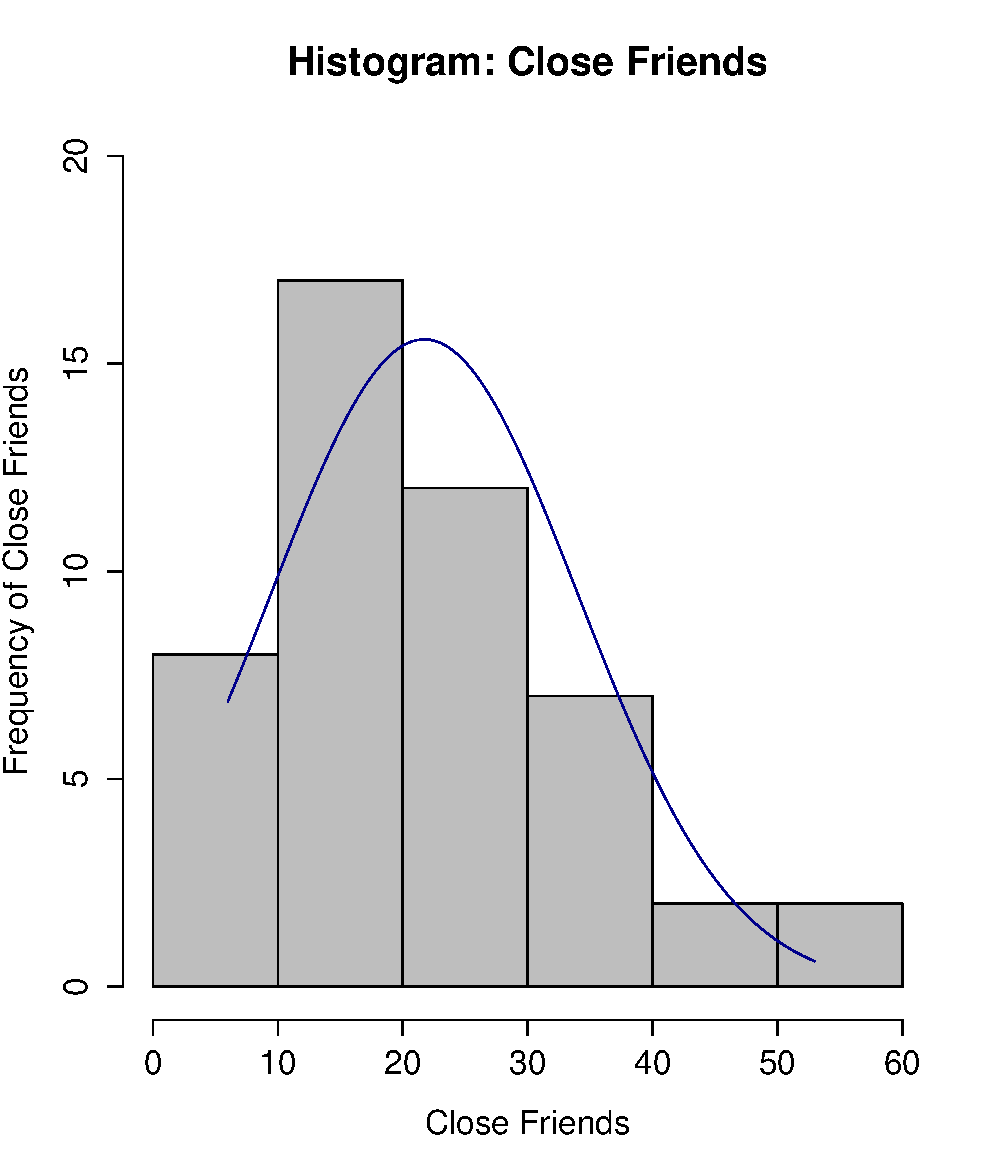
\includegraphics[scale=0.35]{./img/hist_closefriends.pdf}
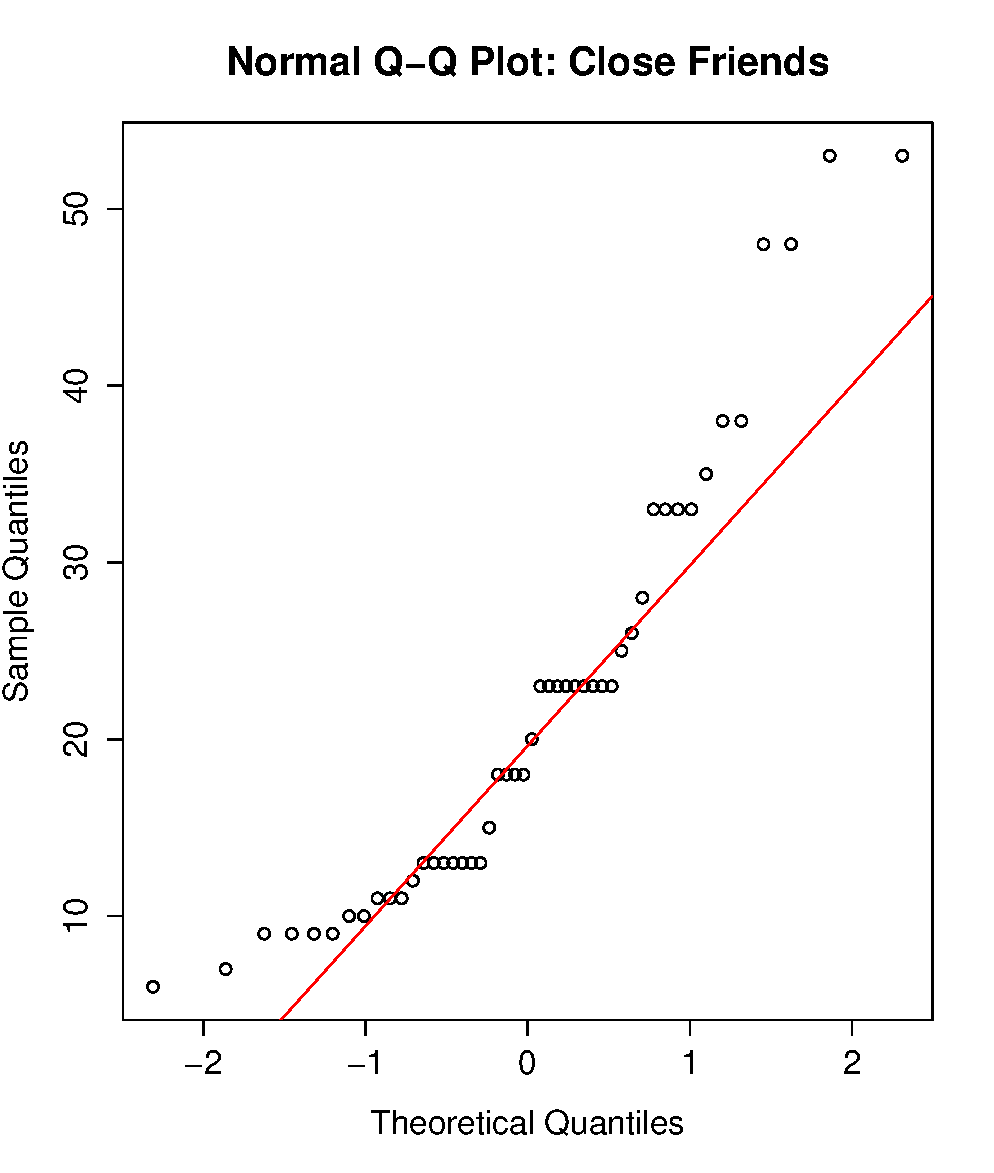
\includegraphics[scale=0.35]{./img/qqplot_closefriends.pdf}
\end{figure}

\subsubsection{Sociability}

Figure 4 shows the histogram and normal q-q plot for Sociability. The blue curve overlay on the histogram demonstrates a non-normal distribution. The normal q-q plot also demonstrates a non-normal distrbution, as the majority of data-points do not fall on the expected normal distribution line. Only non-parametric tests are applicable for this variable.

\begin{figure}[H]
\caption{Histogram and Normal Q-Q Plot: Sociability}
\centering
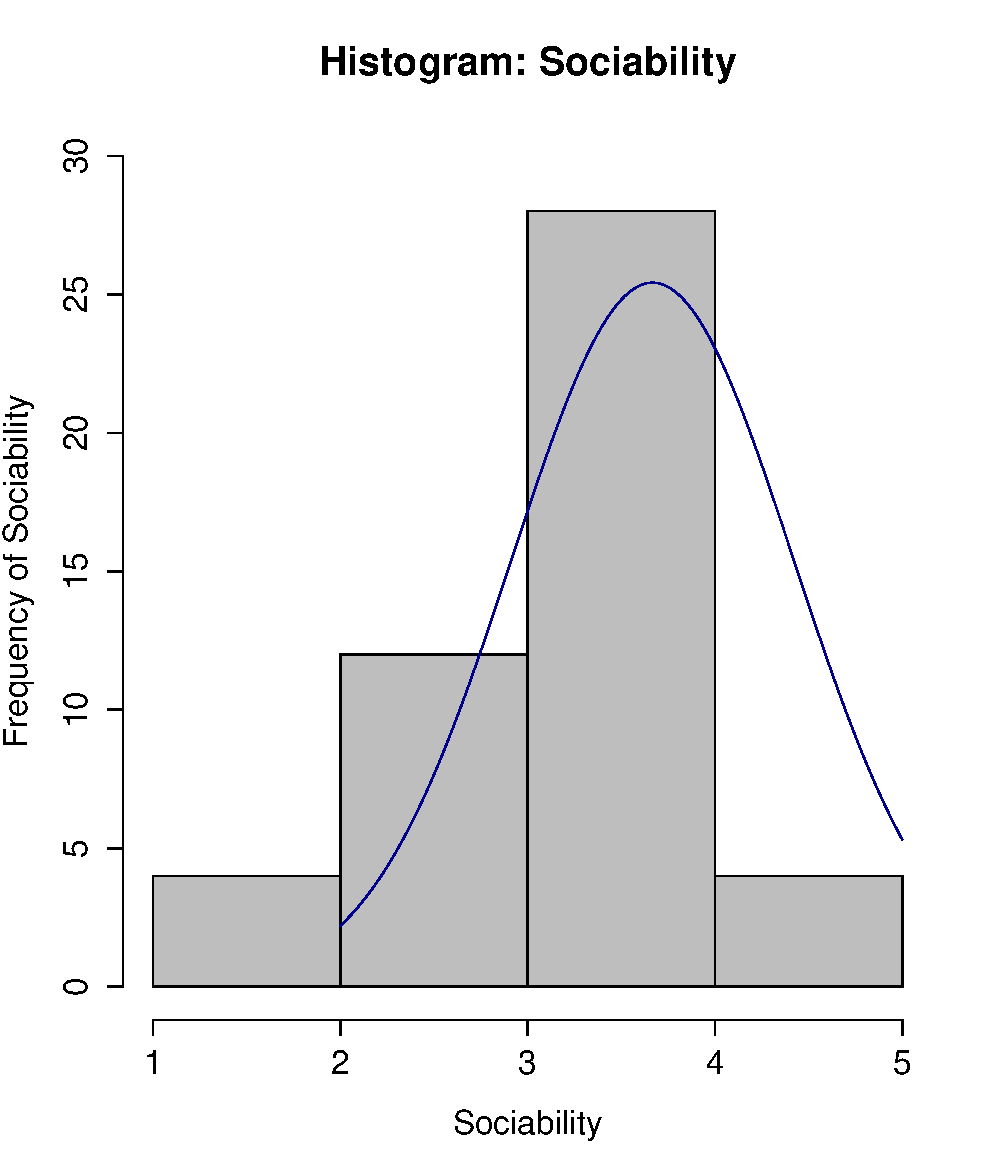
\includegraphics[scale=0.35]{./img/hist_sociability.pdf}
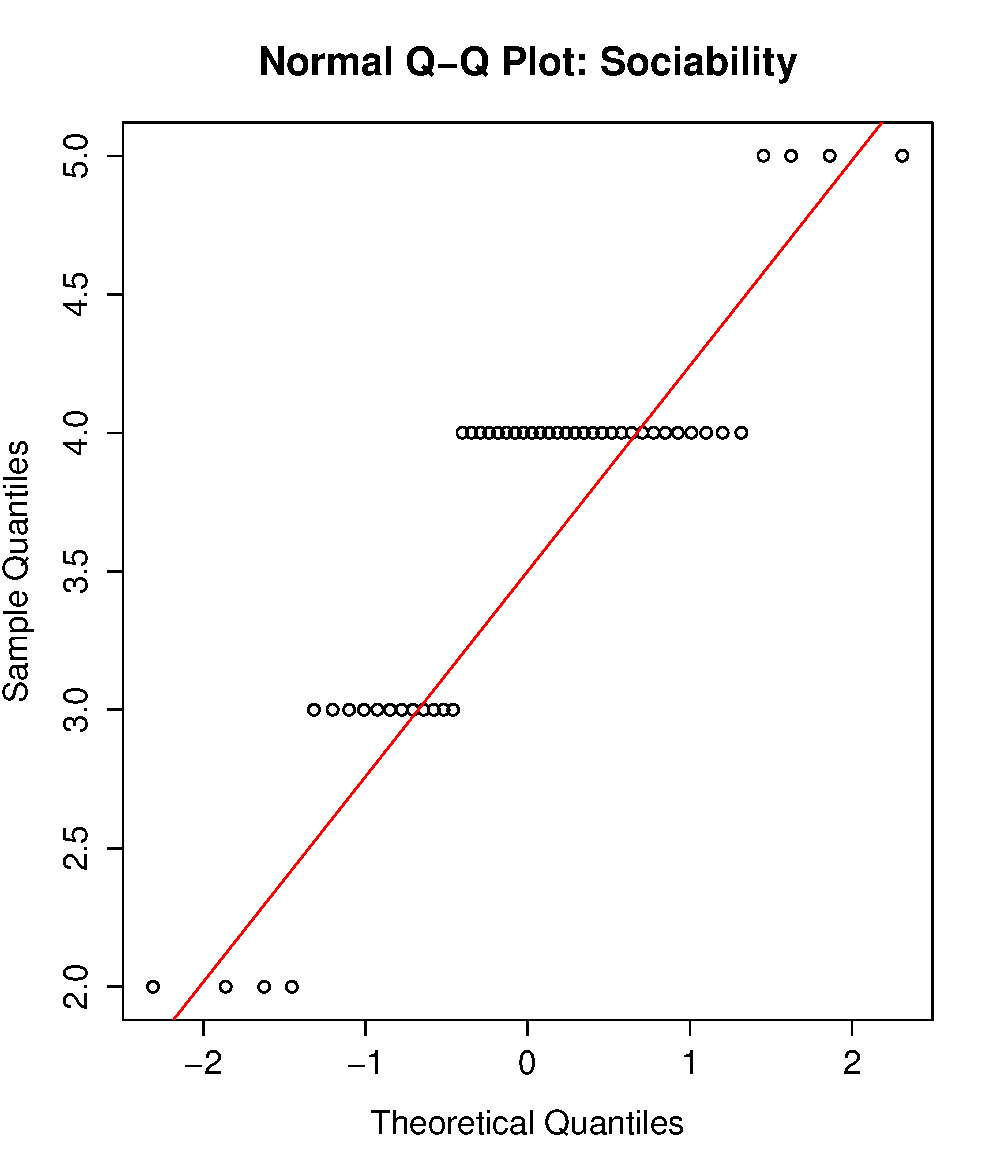
\includegraphics[scale=0.35]{./img/qqplot_sociability.pdf}
\end{figure}

\subsubsection{Facebook hours}

Figure 5 shows the histogram and normal q-q plot for Facebook hours. The blue curve overlay on the histogram demonstrates a non-normal distribution. The normal q-q plot also demonstrates a non-normal distrbution, as the majority of data-points do not fall on the expected normal distribution line. Only non-parametric tests are applicable for this variable.

\begin{figure}[H]
\caption{Histogram and Normal Q-Q Plot: Facebook hours}
\centering
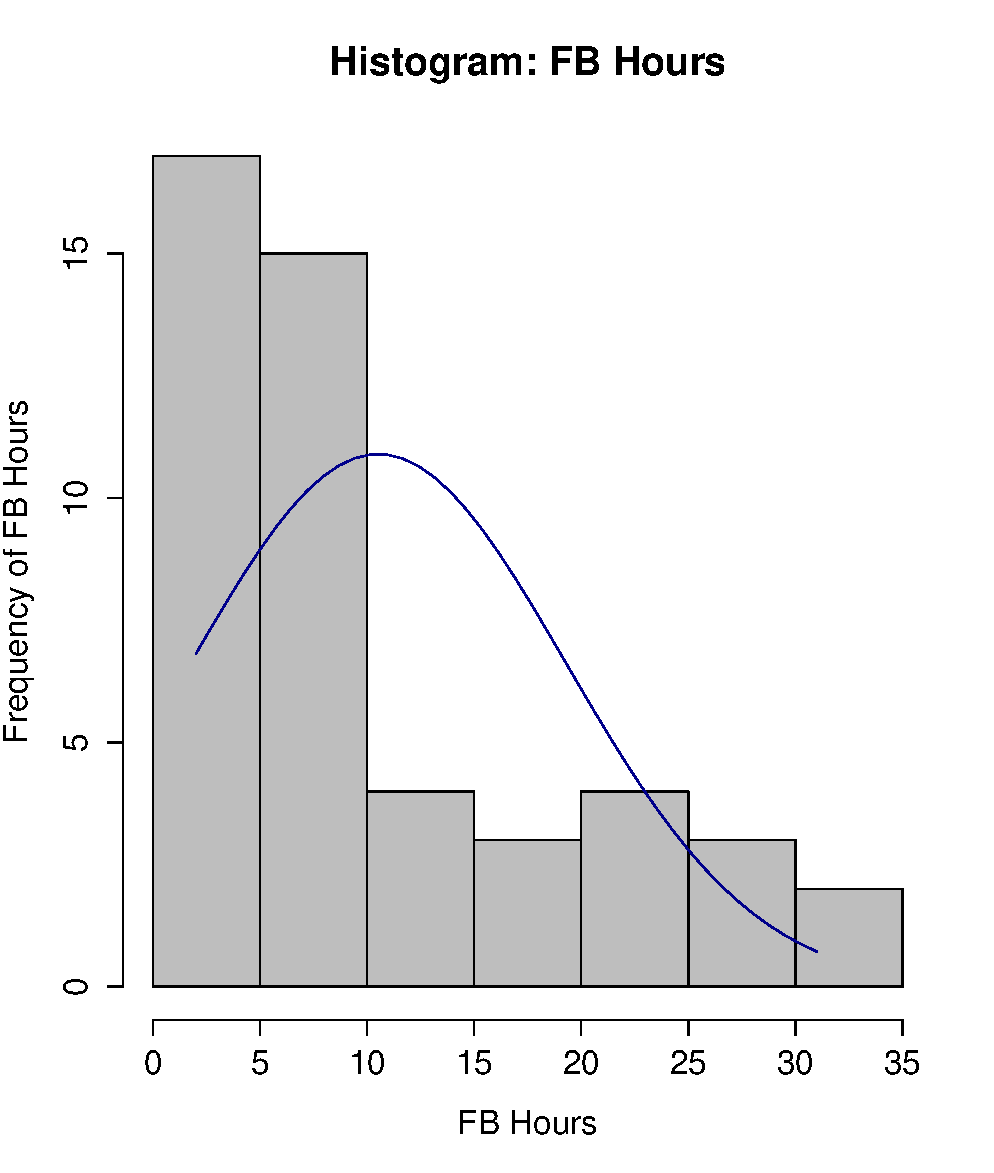
\includegraphics[scale=0.35]{./img/hist_fbhours.pdf}
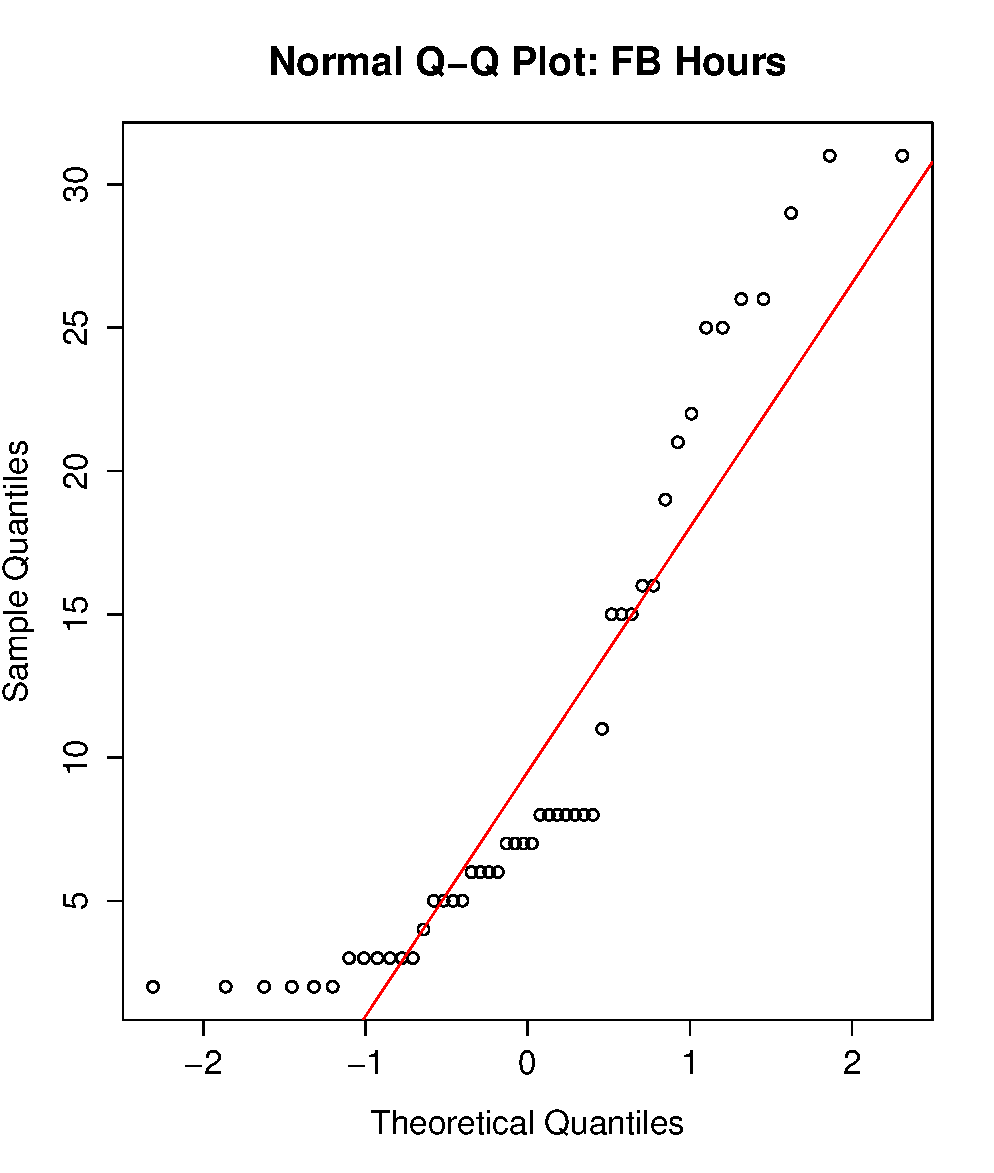
\includegraphics[scale=0.35]{./img/qqplot_fbhours.pdf}
\end{figure}

\subsection{Bivarial inferential tests}

\subsubsection{Pearson's correlation coefficient}

Table 2 displays the Pearson correlation coefficient results with each variable compared with gender. With gender as the $x$ variable, negative $r$ values denote that Facebook friends, close friends and Facebook hours increase in a reverse slope towards 0, which represents women, and conversely decreases towards 1, which represents men. The 0 $r$ value for Sociability indicates that there is no relationship between gender and sociability. These results are also illustrated in the scatter plots from Figure 6 which show the calculated regression line.

Hypothetically, if there were an equal to almost equal ratio between men and women in the dataset, and all variables were of normal distribution, a fair conclusion of these results would be that there is some correlation between gender and the number of Facebook friends, the number of close friends and hours spent on Facebook, and that there are no correlations between gender and Sociability. However, since there is such a small representation of women in the sample set, there is insufficient evidence to provide any meaningful conclusion with the results below.

The variables calculated are non-normally distributed and the results will be further verified by a non-parametric test.

\begin{table}[H]
\centering
\caption{Pearson's correlation coefficient - Gender}
\begin{tabular}{l|l}
Variable      & $r$         \\ \hline
FB Friends    & -0.3176993  \\ \hline
Close Friends & -0.07652931 \\ \hline
Sociability   & 0           \\ \hline
FB Hours      & -0.2815223  \\ \hline
\end{tabular}
\end{table}

\begin{figure}[H]
\caption{Scatter Plots}
\centering
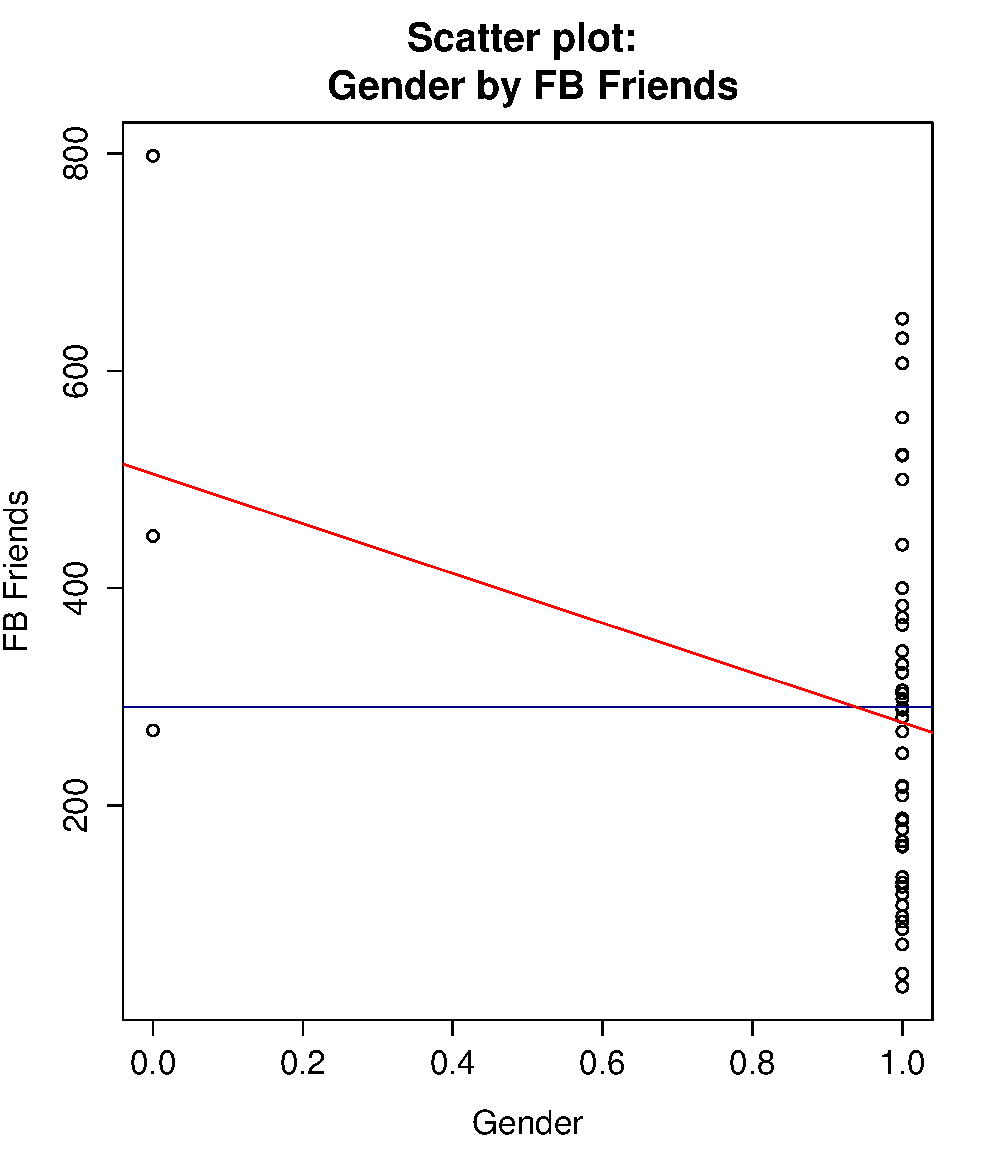
\includegraphics[scale=0.44]{./img/scatplot_fbfriends.pdf}
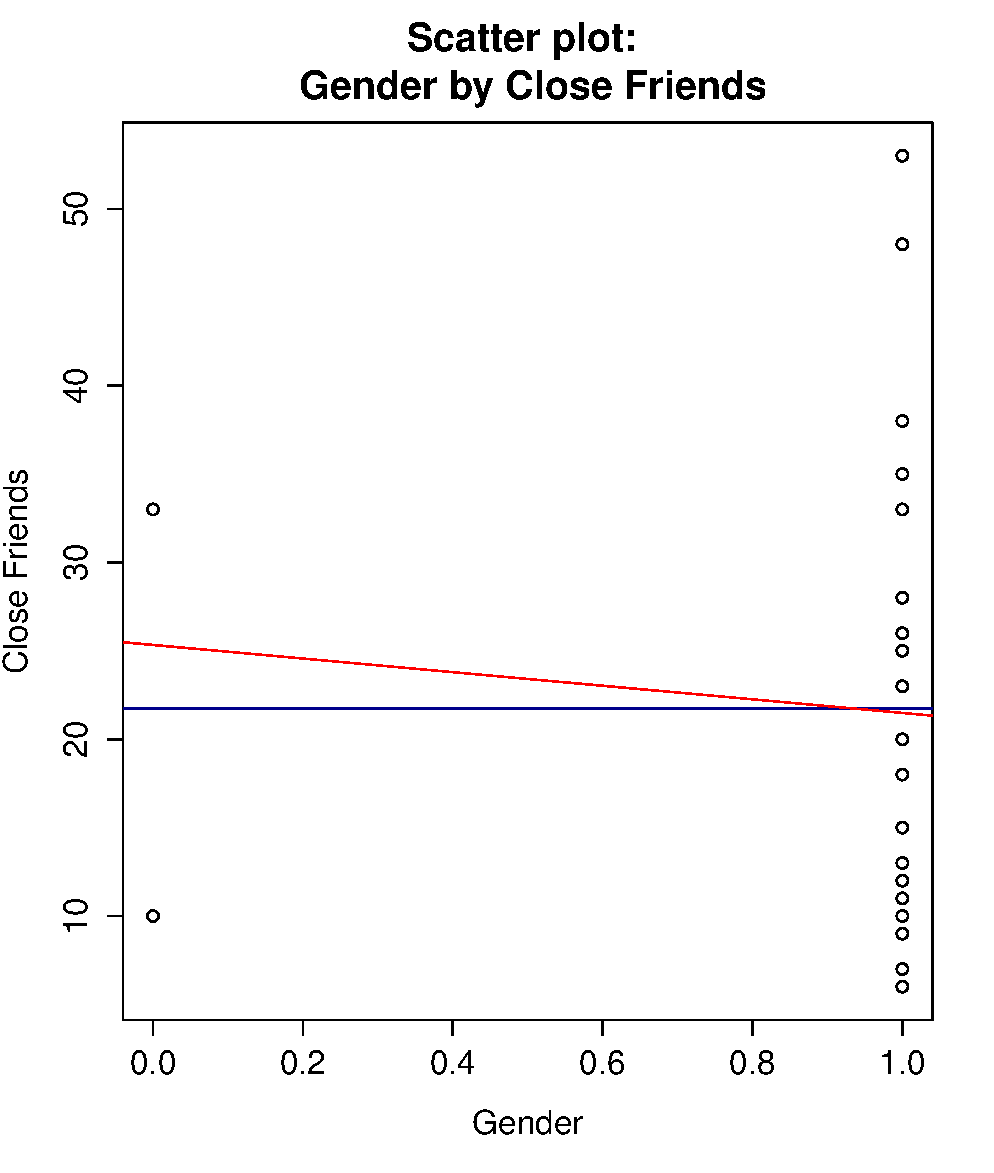
\includegraphics[scale=0.44]{./img/scatplot_closefriends.pdf}
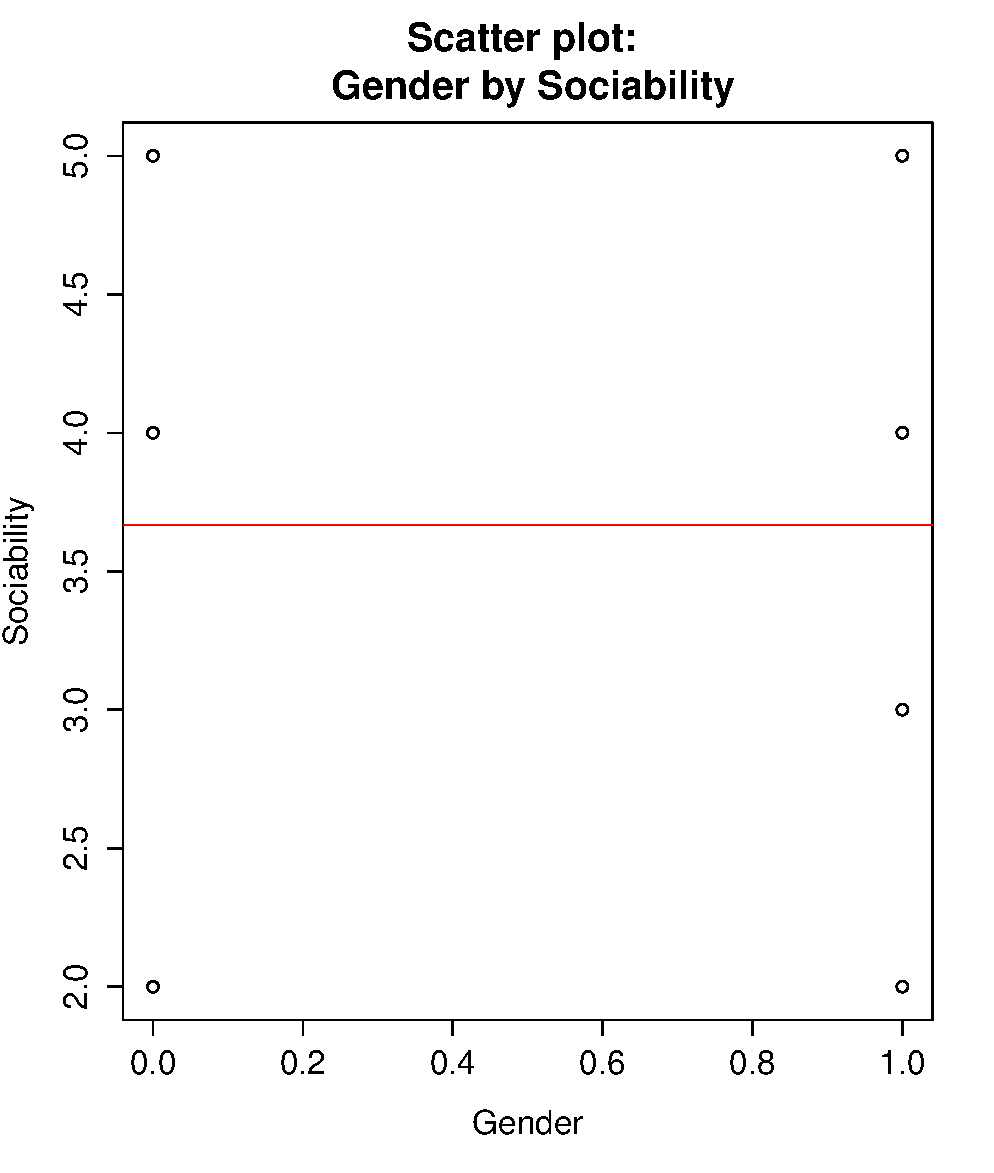
\includegraphics[scale=0.44]{./img/scatplot_sociability.pdf}
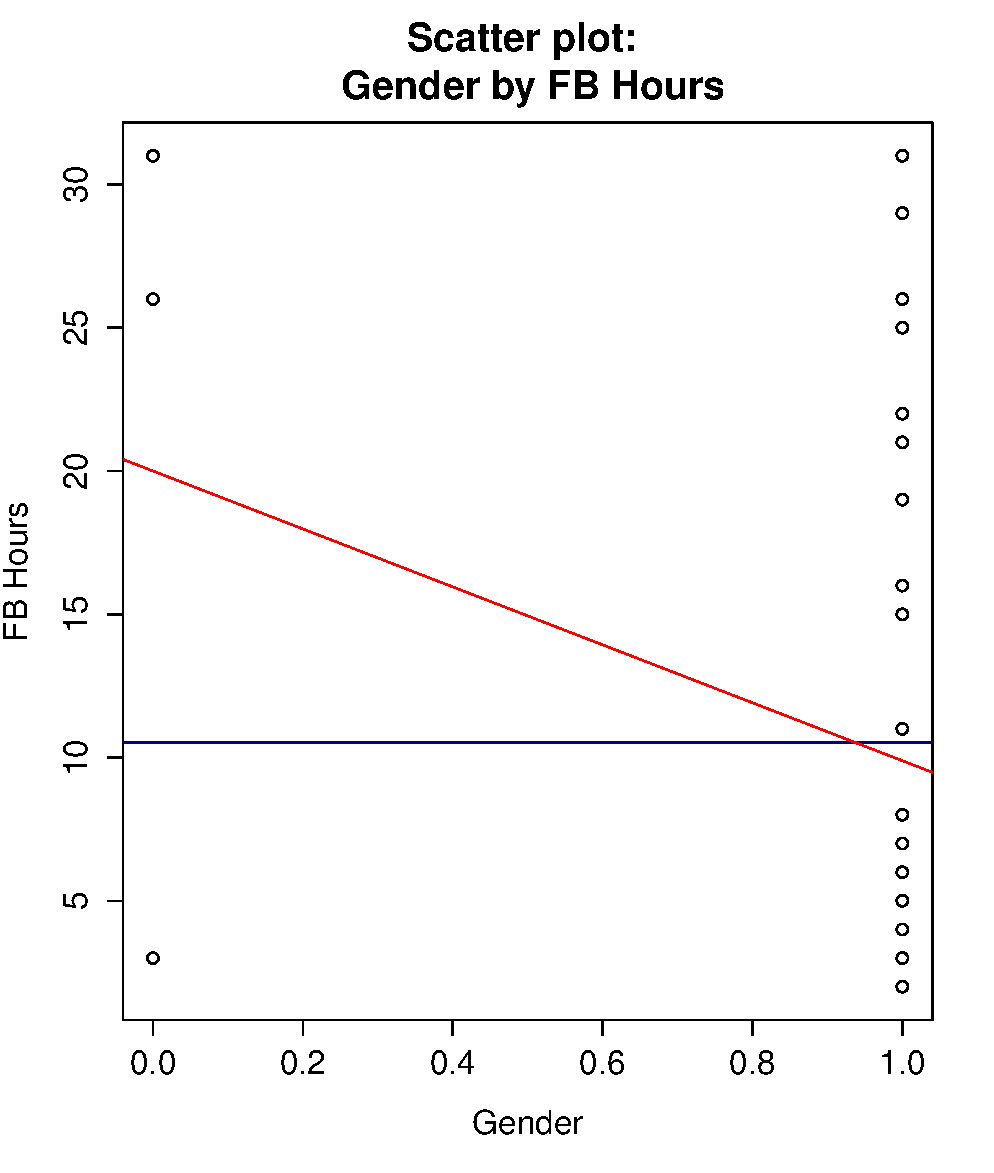
\includegraphics[scale=0.44]{./img/scatplot_fbhours.pdf}
\end{figure}

\newpage
\subsection{Spearman's correlation coefficient}

Table 3 displays the Spearman's correlation coefficient results with each variable compared with gender. Similar results are found, calculating the correlation coefficient using Spearman's method. However, in this instance, a small correlation value is found for gender and Sociability.

As all the variables being calculated are non-normally distributed, these $r$ values generated by a non-parametric test can be regarded with higher reliability. However, the same issue still applies, in that women are under represented in the sample set, and there is not enough evidence to provide any meaningful conclusions.

\begin{table}[H]
\centering
\caption{Spearman's correlation coefficient - Gender}
\begin{tabular}{l|l}
Variable      & $r_s$         \\ \hline
FB Friends    & -0.2391999  \\ \hline
Close Friends & -0.08123761 \\ \hline
Sociability   & -0.04207032 \\ \hline
FB Hours      & -0.1747336  \\ \hline
\end{tabular}
\end{table}